\documentclass[svgnames,smaller,10pt]{beamer}

\usetheme{metropolis}

\usepackage[utf8]{inputenc}
\usepackage[french]{babel}
\usepackage{hyperref}
\hypersetup{
    unicode=true,          
    psdextra=true,         % Aide à mieux interpréter certains symboles
    pdfencoding=auto,
}
\usepackage[T1]{fontenc}
\usepackage{geometry}
\geometry{
    left=2.5mm,
    right=2.5mm,
    top=0mm,
    bottom=0mm
}
\usepackage{amssymb} % pour \blackdiamond
\usepackage{tikz}
\usepackage{graphicx,animate}
\usepackage{subcaption}


\newcommand{\replacementchar}{%
  \tikz[baseline=-0.6ex]{
    %\node[inner sep=0pt] (d) {\Large$\blackdiamond$};
    \node[inner sep=0pt] (d) {\Large$\blacksquare$};
    \node[white, font=\scriptsize\bfseries] at (d.center) {?};
  }%
}
\usepackage{tabularx}
%\usepackage[style=alphabetic,citestyle=authoryear]{biblatex}
%\addbibresource{bibliographie.bib}

\usepackage{xspace}
\newcommand{\themename}{\textbf{\textsc{metropolis}}\xspace}
\title{L2S4: Édition numérique\\
TD 7: A-t-on encore besoin des éditeurs-rices à l'heure de l'édition numérique ?
\\
\small
Auto-édition, désintermédiation et réintermédiation
}

\date{}
\author{Marine Tiger\\   \texttt{marine.tiger@sorbonne-universite.fr}}

\institute{Littératures françaises et comparée ED19, CELLF, Sorbonne Université}

\begin{document}
\maketitle
\setbeamertemplate{section in toc}[sections numbered]

\section{Introduction}
\begin{frame}{Introduction}
\begin{figure}
    \centering
    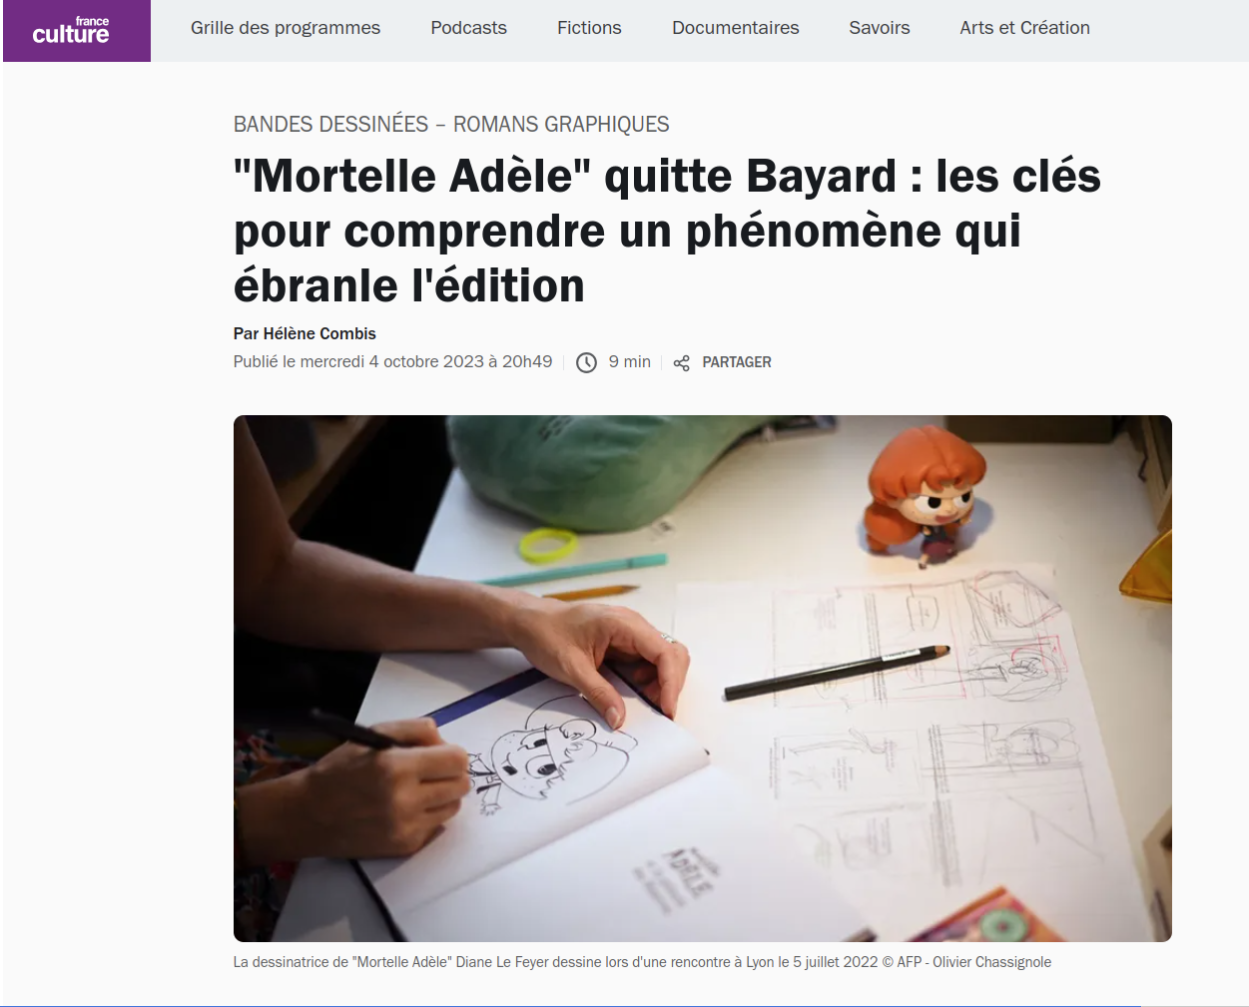
\includegraphics[width=0.80\textwidth]{images/mortelle_adele.png}
\end{figure}

\end{frame}

\begin{frame}{Quelques chiffres}
    \begin{columns}
        % Colonne de gauche : Texte
        \begin{column}{0.4\textwidth}
            Sur 70087 auteur.rices ayant déposé au moins un livre à la BnF entre 2007 et 2016:
            \begin{itemize}
                \item 48\% sont toujours restés fidèles à l'édition classique
                \item 40\% n'ont jamais quitté l'auto-édition.
                \item \textbf{12\% sont passés de l'un à l'autre} entre 1970 et 2016
            \end{itemize}
        \end{column}

        % Colonne de droite : Image
        \begin{column}{0.5\textwidth}
            \centering
            
\includegraphics[width=.80\columnwidth]{images/autoedition-rapport.png}
        \end{column}
    \end{columns}
\end{frame}

\begin{frame}{Quelques chiffres}
    L'auto-édition, c'est\dots
    \begin{itemize}
        \item 20\% des oeuvres déposées au dépôt légal en 2019 (contre 12\% en 2010);
        \item 60\% des livres de poésie en 2015;
        \item une surreprésentation aussi des romans: 25\% des livres enregistrés au dépôt légal.
    \end{itemize}

Mais aussi\dots
\begin{itemize}
    \item Des startégies éditoriales variées;
    \item Un parcours encore difficile;
    \item Un désir d'émancipation
\end{itemize}
\end{frame}

\begin{frame}{Problématique}
    \centering
    Quel est le rôle joué par les technologies numériques dans ces pratiques d'auto-édition ?
\end{frame}



\section{Auto-édition: de quoi parle-t-on?}
\begin{frame}{Les notions abordées}
    \begin{itemize}
        \item Auto-édition
        \item Auto-publication
        \item Publications à compte d'auteur
    \end{itemize}
\end{frame}

\begin{frame}{Publication à compte d'auteur}
    Consiste pour un auteur à faire éditer ses propres ouvrages \textbf{par un éditeur qui assure seulement la partie technique de l'édition et de la diffusion.}\\
    \textrightarrow{} L'auteur paie les frais d'impression et de publicité mais reste propriétaire de ses droits d'auteur.\\
\end{frame}

\begin{frame}{Publication à compte d'auteur}
    \begin{columns}
    % Colonne de gauche : Texte
        \begin{column}{0.4\textwidth}
            \begin{itemize}
                \item Système inventé par \textbf{Bernard Grasset}.
                \item Créateur du marketing éditorial.
                \item Exemple de Proust en 1913: 1250 exemplaires du premier tome sont imprimés.
            \end{itemize}
        \end{column}

        % Colonne de droite : Image
        \begin{column}{0.5\textwidth}
            \centering
            
\includegraphics[width=.70\columnwidth]{images/Proust_1913.jpg}
        \end{column}
    \end{columns}
\end{frame}

\begin{frame}{Publication à compte d'auteur}
    \begin{itemize}
        \item \textbf{Le texte ne passe pas devant un comité de lecture} mais intègre tout de suite le circuit de fabrication;
        \item \textbf{L'éditeur n'assume pas le risque éditorial} \textrightarrow{} En contrepartie, l’auteur ne lui cède pas ses droits;
        \item \textbf{L'écrivain ne bénéficie pas tout à fait de la fonction de légitimation}: pas d'approbation d'un comité éditorial mais bénéficie des compétences techniques de fabrication du livre et de l'énonciation éditoriale.
    \end{itemize}

\end{frame}

\begin{frame}{Publication à compte d'auteur}
    \begin{columns}
    % Colonne de gauche : Texte
        \begin{column}{0.4\textwidth}
            \begin{itemize}
                \item Harmattan: fondée en 1975;
                \item Publication d'ouvrage d'auteurs africains ou tiers-mondistes;
                \item Permet d'éditer son livre gratuitement mais ne verse des droits d'auteurs qu'à partir du 500ème livre vendu.
            \end{itemize}
        \end{column}

        % Colonne de droite : Image
        \begin{column}{0.5\textwidth}
            \centering
            
\includegraphics[width=\textwidth]{images/harmattan.png}
        \end{column}
    \end{columns}
\end{frame}

\begin{frame}{Auto-publication}
    Consiste à rendre public un texte, sans nécessairement cherche à le commercialiser.\\
    \textrightarrow{} Impact du développement du web à compter des années 1990.
\end{frame}
\begin{frame}{Auto-publication et édition numérique : naissance d'une nouvelle avant-garde littéraire}
    Rappel:
    \begin{itemize}
        \item Web = application d'internet, qui propose une infrastructure en réseau et permet de publier des contenus de tous types.
        \item Textes publiés sur le Web dès les années 90 sont des textes encodés dans des formats numériques: XML, HTML.
    \end{itemize}
    \textbf{Naissance d'un web littéraire \textrightarrow{} avant-garde littéraire:}
    \begin{itemize}
        \item Écrivains des débuts du web doivent apprendre des langages de programmation.
        \item Vont créer des oeuvres littéraires qui reposent non seulement sur le langage naturel, mais aussi sur une exploitation du langage de progammation.
    \end{itemize}
    
\end{frame}

\begin{frame}{Des outils pour l'auto-publication}
    \begin{columns}
    % Colonne de gauche : Texte
        \begin{column}{0.4\textwidth}
            \begin{itemize}
                \item Années 2000: multiplication d'outils de publication;
                \item Directement possible de publier un contenu sur le web sans connaître HTML, CSS ou Javascript.
            \end{itemize}
        \end{column}

        % Colonne de droite : Image
        \begin{column}{0.5\textwidth}
            \centering
            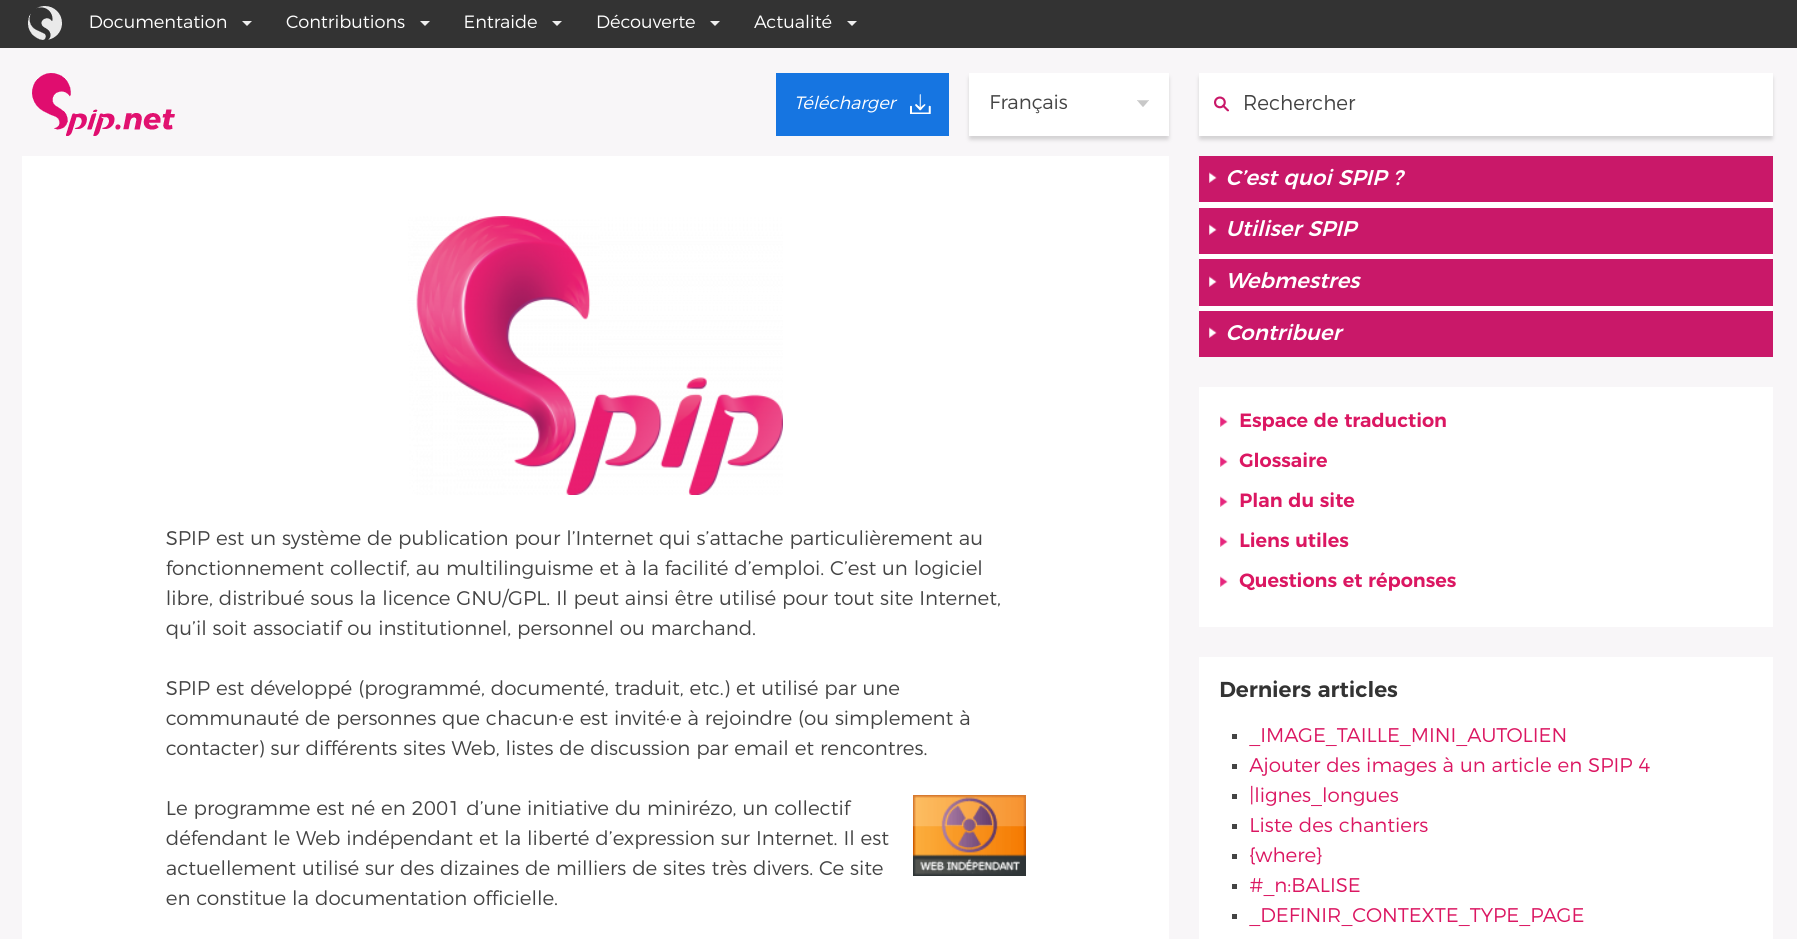
\includegraphics[width=\textwidth]{images/spip1.png}
        \end{column}
    \end{columns}
\vspace{2em}
\textbf{Sur la souveraineté des outils:} question des modèles économiques de l'édition numérique (les GAFAM) \textrightarrow{} Nouveau monopole éditorial qui ne rémunère pas ce qui est publié par exemple. 
\end{frame}
\begin{frame}{Les "plateformes littéraires"}
    \begin{columns}
    % Colonne de gauche : Texte
        \begin{column}{0.4\textwidth}
            \begin{itemize}
                \item Plateformes dédiées de type Wattpad;
                \item Des outils de plus en plus formattés;
                \item Des degrès de "professionnalisme" variables. Wattpad revendique l'amateurisme par exemple.
            \end{itemize}
        \end{column}

        % Colonne de droite : Image
        \begin{column}{0.5\textwidth}
            \centering
            
\includegraphics[width=\textwidth]{images/wattpad.png}
        \end{column}
    \end{columns}
\end{frame}

\begin{frame}{Les "plateformes littéraires"}
    \begin{columns}
    % Colonne de gauche : Texte
        \begin{column}{0.4\textwidth}
            \begin{itemize}
                \item écosystèmes de publication: kindle direct publishing, kobo writing life, iBooks authors\dots
                \item Ne demandent aucune contribution financière à l’auteur mais le travail éditorial n'est pas pris en charge.
            \end{itemize}
        \end{column}

        % Colonne de droite : Image
        \begin{column}{0.5\textwidth}
            \centering
            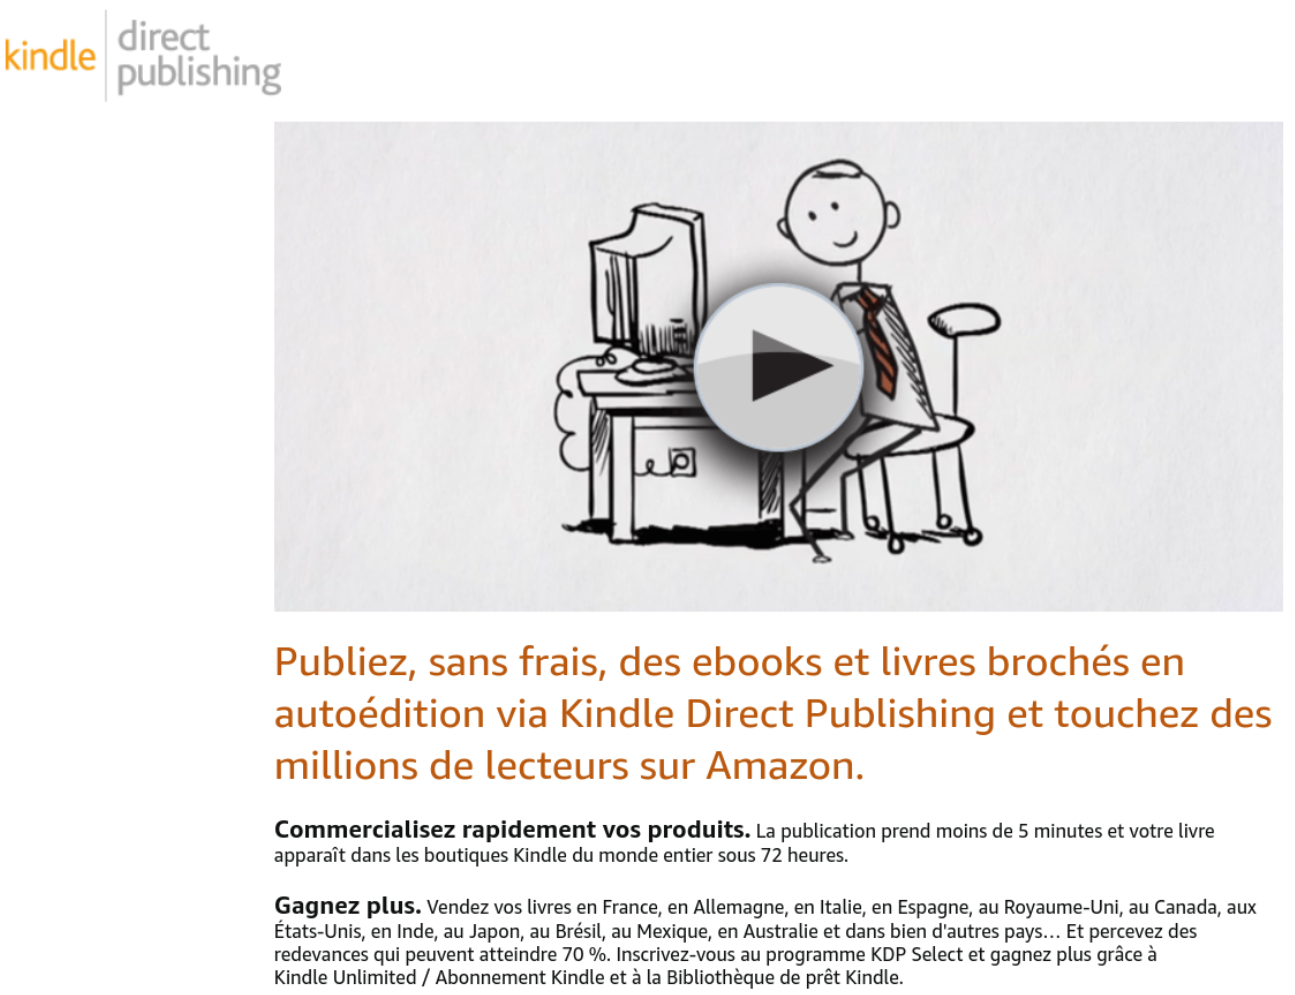
\includegraphics[width=\textwidth]{images/kindle_publishing.png}
        \end{column}
    \end{columns}
    
\end{frame}

\begin{frame}{Quelques \textit{success stories} qui alimentent les fantasmes}
    \begin{figure}
        
\includegraphics[width=.60\textwidth]{images/AgnesMartinLugand.png}
    \end{figure}
    
\end{frame}
\begin{frame}{Quelques \textit{success stories} qui alimentent les fantasmes}
    \begin{columns}
    % Colonne de gauche : Texte
        \begin{column}{0.4\textwidth}
            \begin{itemize}
                \item Exemple d'éditeurs-diffuseurs numériques: Librinova.
                \item Propose contre rémunération un accompagnement de l'auteur sous la forme de prestations professionnelles.
            \end{itemize}
        \end{column}

        % Colonne de droite : Image
        \begin{column}{0.5\textwidth}
            \centering
            
\includegraphics[width=\textwidth]{images/librinova.png}
        \end{column}
    \end{columns}
    
\end{frame}
\begin{frame}{Auto-édition}
    Renvoie à un modèle d'auto-publication: 
    \begin{itemize}
        \item qualitatif
        \item Modèle éditorial traditionnel
        \item Souvent une vocation marchande.
    \end{itemize}
    
\end{frame}
\begin{frame}{Exemple: Tiers Livre éditeur de François Bon}
    \begin{figure}
        \centering
        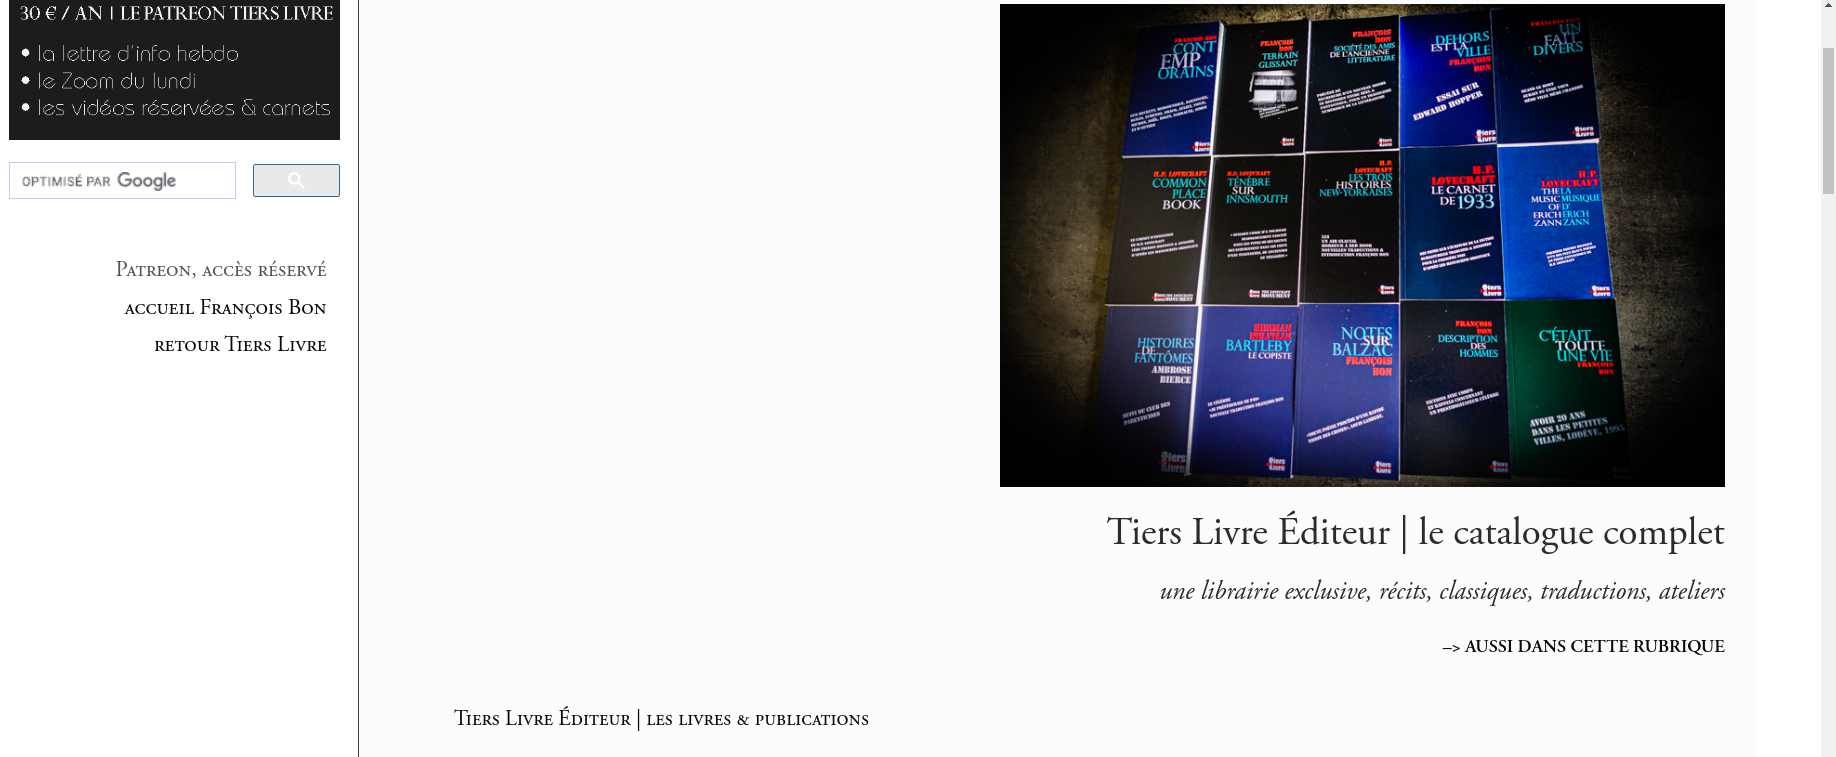
\includegraphics[width=.4\textwidth, height=3cm]{images/FBediteur.png}
        \hspace{1em}
        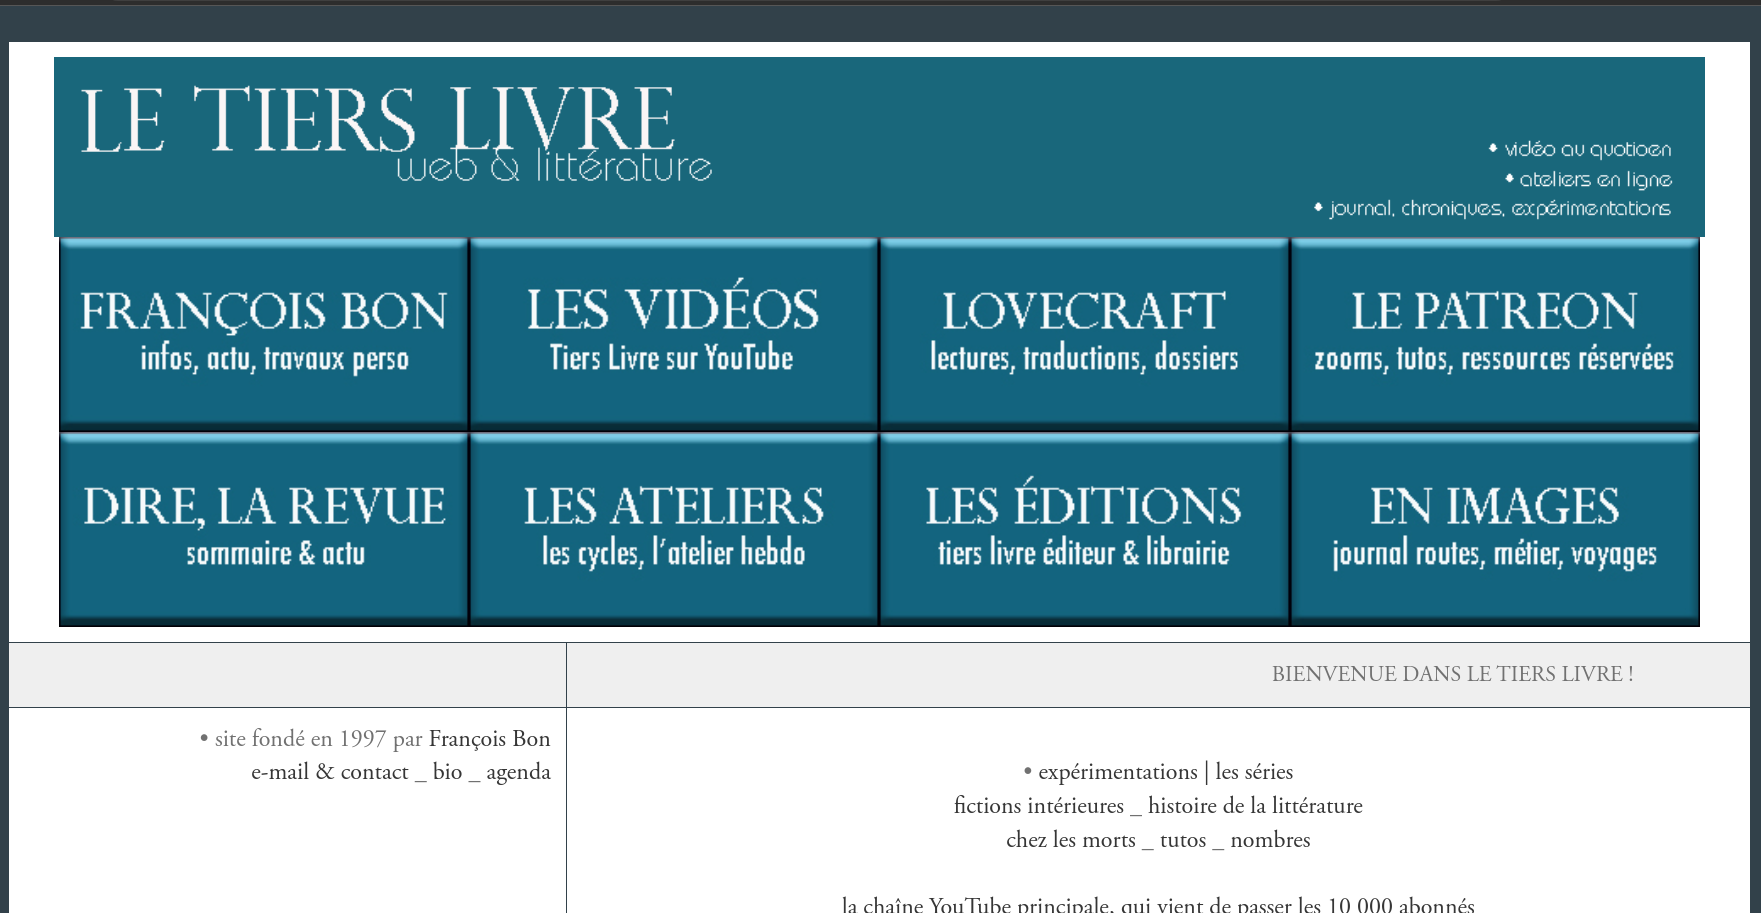
\includegraphics[width=.4\textwidth]{images/FBediteur2.png}
    \end{figure}
\end{frame}

\begin{frame}{Autre exemple: Pierre Ménard de La Marelle au livre-objet auto-édité}
    \begin{figure}
        \centering
        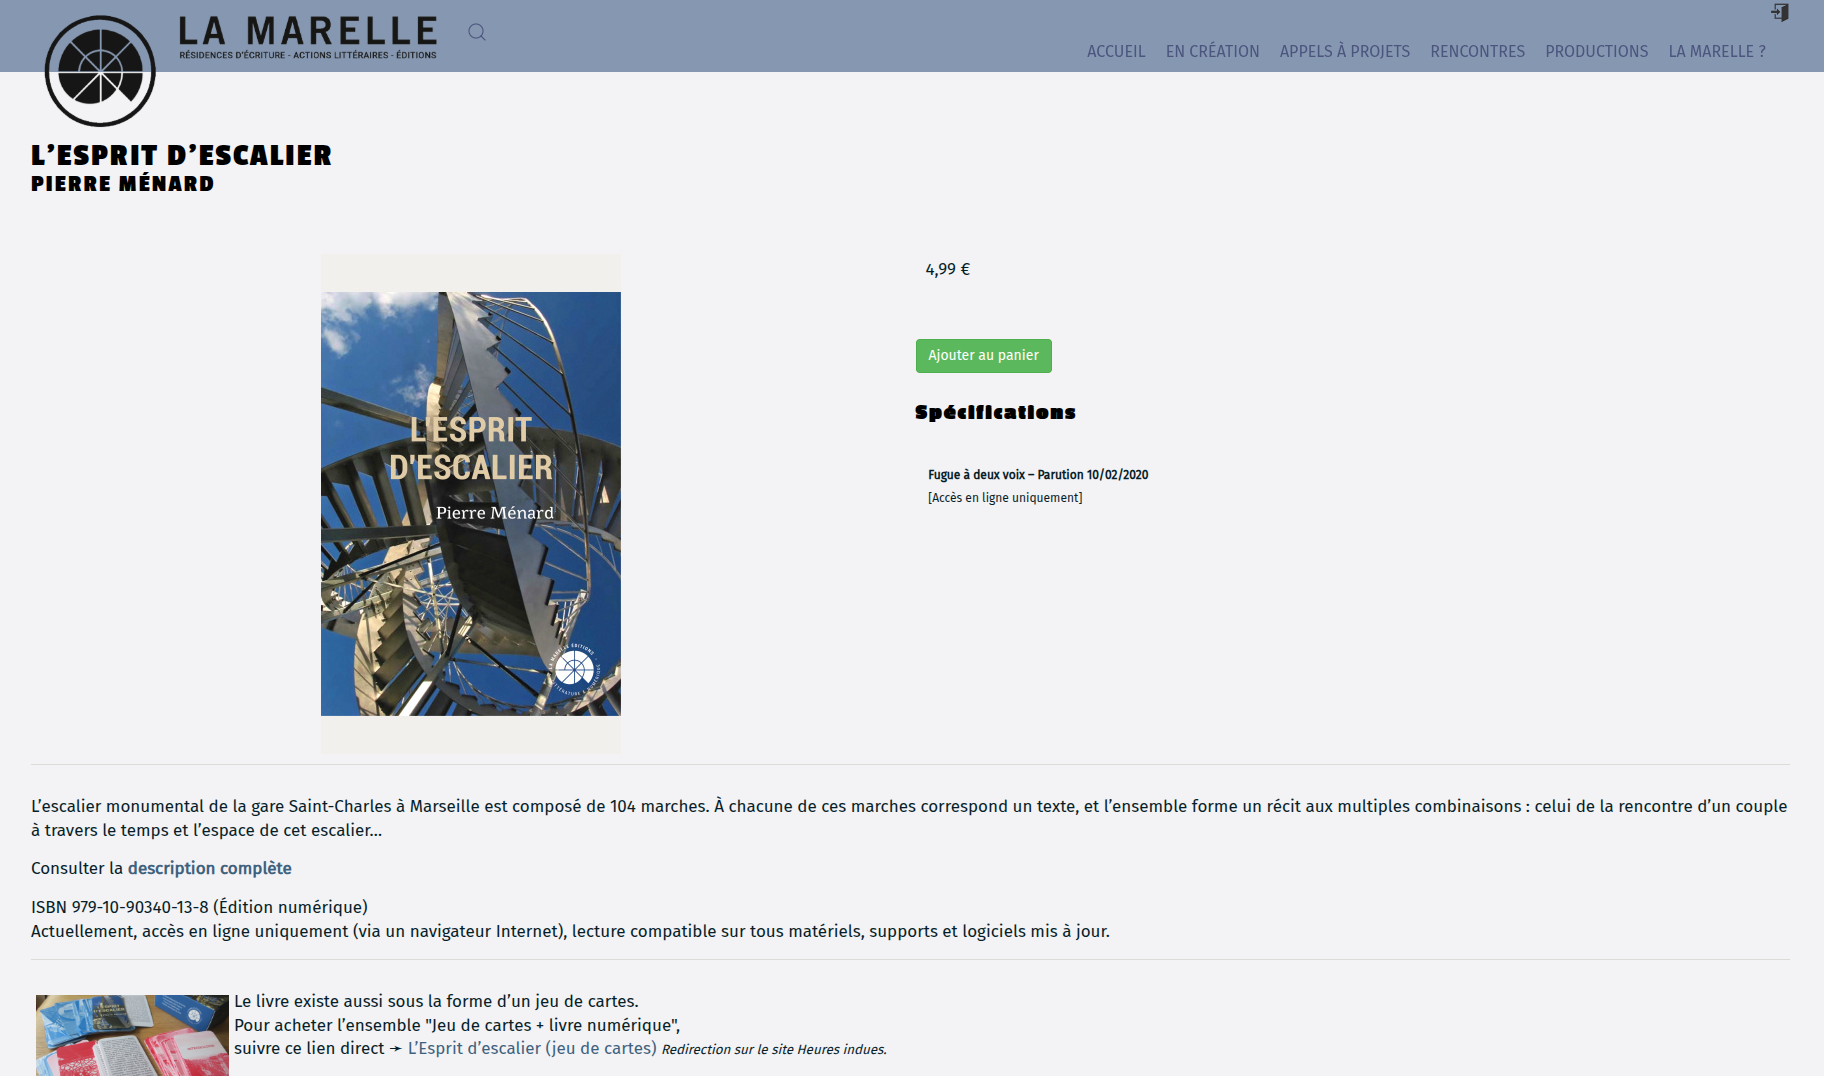
\includegraphics[width=.4\textwidth]{images/espritEscalier.png}
        \hspace{1em}
        
\includegraphics[width=.4\textwidth]{images/heuresIndues.png}
    \end{figure}
\end{frame}

\section{Une édition sans éditeurs-rices ?}
\begin{frame}{La tentation de la désintermédiation}
    \begin{itemize}
        \item Précarisation des écrivain.es 
        \item Tensions avec les grands éditeur.rices 
        \item Mise à disposition d'outils d'auto-publication/édition 
    \end{itemize}
    \textrightarrow{} place de l'éditeur.rice au sein de l'écosystème éditorial?\\
    \vspace{1em}
    \textbf{Concept de la désintermédiation}\\
    Gallezot Gabriel et Ertzscheid Olivier, \textit{« Swaper la publication »}, 2006: "[...] pour l'autopublication, il faut ajouter "sans intermédiaire"" dans le processus de publication.
\end{frame}

\begin{frame}{Qu'entend-t-on par désintermédiation?}
    \begin{enumerate}
        \item Un concept économique dès les années 60 avec le développement de techniques numériques.
        \item Établissement d'une relation directe entre une entité (industrielle, culturelle, institutionnelle) et ses usagers entraînant la disparition de certains services.
    \end{enumerate}
    \textrightarrow{} Renvoie à \textbf{la disparition de certains intermédiaires} qui incarnaient une forme d'autorité, ou qui conféraient cette autorité\\
    = les édteur.rices, les grands distributeurs, les libraires etc...
\end{frame}
\begin{frame}{Exemple: les critiques littéraires}
    \begin{figure}
        \centering
        
\includegraphics[width=.4\textwidth]{images/masque_plume.png}
        \hspace{1em}
        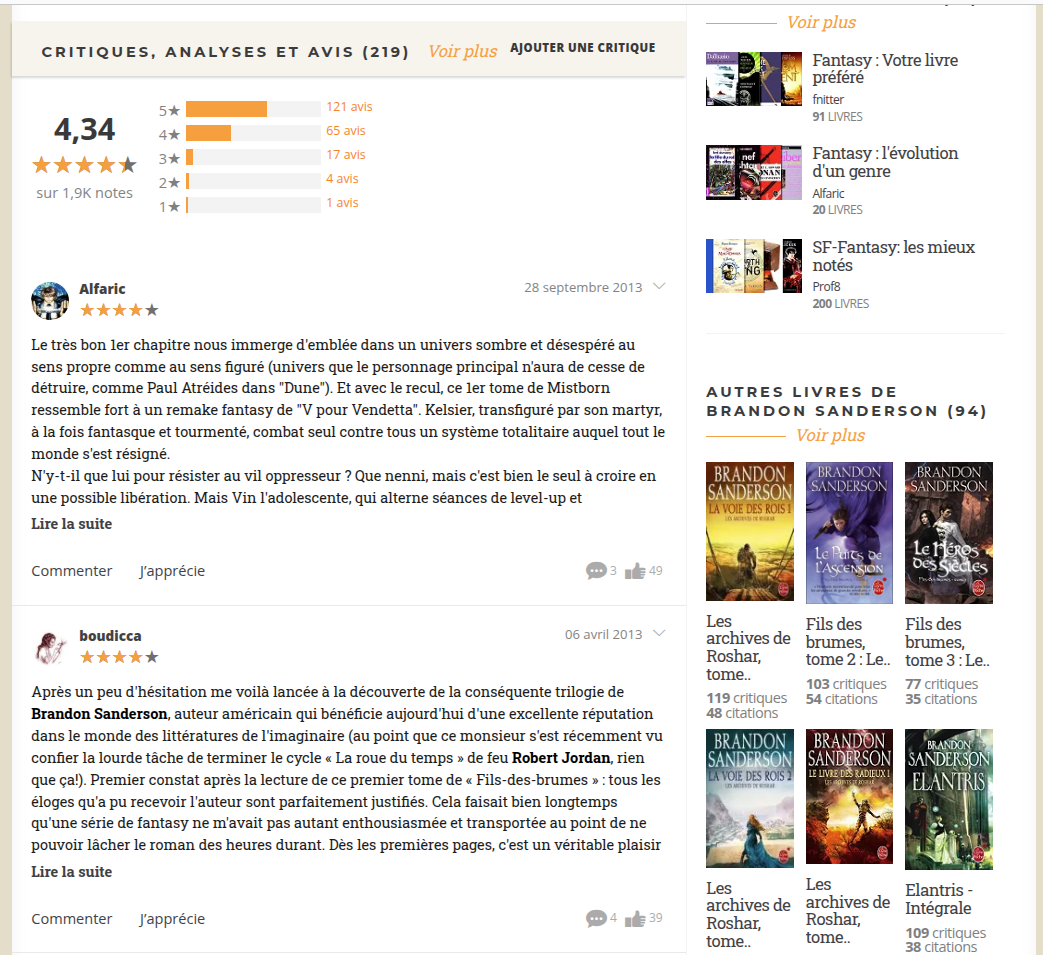
\includegraphics[width=.4\textwidth]{images/babelio.png}
    \end{figure}
\end{frame}
\begin{frame}{Exemple: les critiques littéraires}
    \begin{block}{Booktube, BookTok, Bookstagram}
        \begin{figure}
            \centering
            
\includegraphics[width=.45\textwidth, height=5cm]{images/Bookstagram.png}
            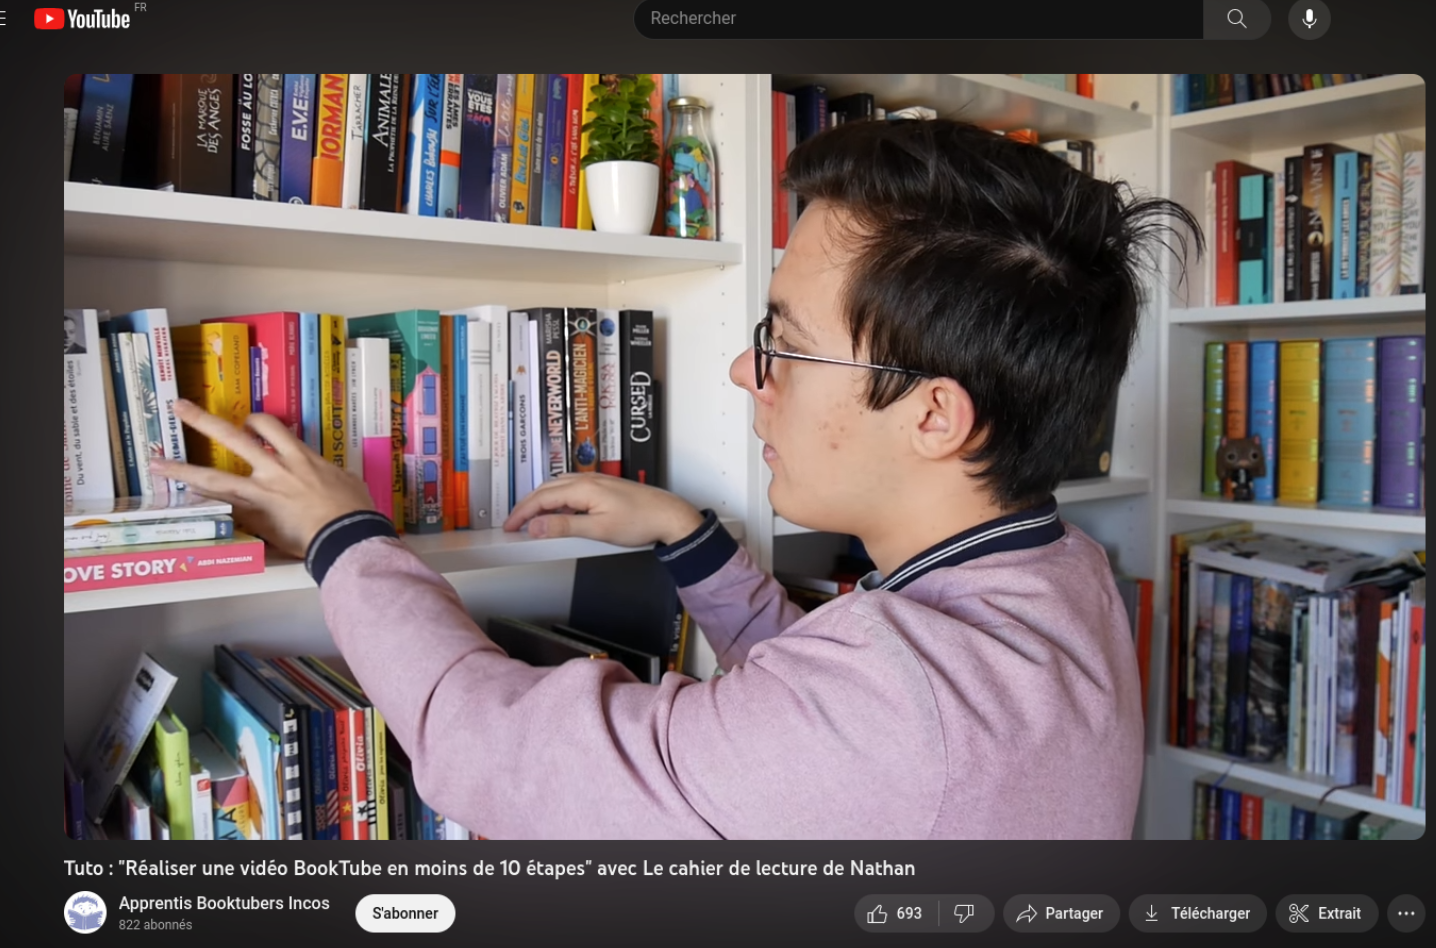
\includegraphics[width=.45\textwidth, height=5cm]{images/BookTube.png}
        \end{figure}
    \end{block}
    
\end{frame}

\begin{frame}{Exemple: les critiques littéraires}
    \begin{figure}
        \begin{center}
            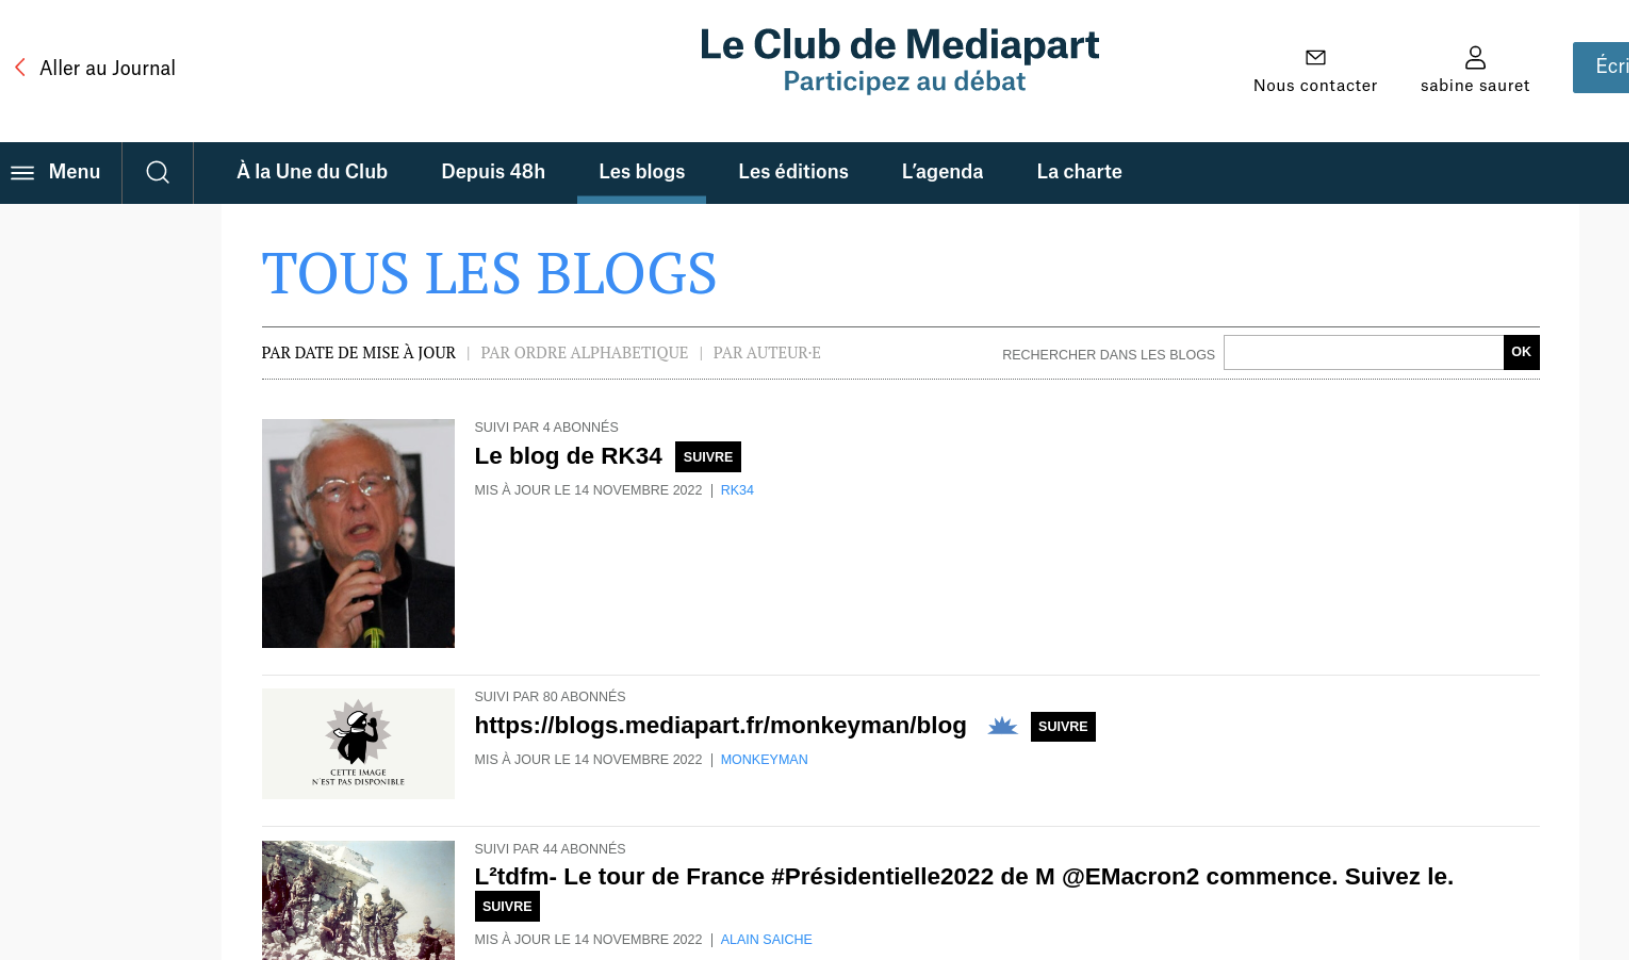
\includegraphics[width=.8\textwidth]{images/mediapart.png}
        \end{center}
    \end{figure}
\end{frame}
\begin{frame}{Remise en question des autorités ayant un fort pouvoir de légitimation}
    Désintermédiation pose de nombreuses questions en termes de système hiérarchique de valeur attribués aux contenus.
\end{frame}

\section{La désintermédiation et l'informatisation}
\begin{frame}{De l'automatisation des tâches à la menace de l'obsolescence des métiers techniques de la culture}
    Concept dont on discute depuis les années 1960, avec le développement de dispositifs techniques (en particulier l'informatique) \textrightarrow{} Automatisation de certaines tâches jusque-là assurées par des être humains.\\
    \vspace{1em}
Essayer de proposer de nouveaux services et donc une nouvelle manière de concevoir leur métier / le service ou l'objet qu'ils vendaient.\\
\textbf{Exemple:  }\\

\end{frame}

\begin{frame}{Exemple: l'informatisation du catalogue à la BnF}
    \textbf{Documentaire sur la BnF d'Alain Resnais, \textit{Toute la mémoire du monde}}\\
    \url{https://cours-edition-litterature-numerique-l2-92cac3.gitpages.huma-num.fr/img/Resnais_extrait.mp4}\\
    \vspace{1em}
    \pause
    \begin{itemize}
        \item Sous forme de fiches dans des catalogues imprimés;
        \item Pour Éric de Grolier (éditeur, chercheur, parfois considéré comme le fondateur des sciences de l'information en France), le documentaliste = « intermédiaire dont la fonction essentielle est de mettre en contact ceux qui ont besoin de savoir et ceux qui savent »
        \item Ailleurs on parle d’un « médiateur entre le document et l’utilisateur ».
        \item Gain d'autonomie énorme pour le lecteur
    \end{itemize}
    Reportage France 2: \url{https://cours-edition-litterature-numerique-l2-92cac3.gitpages.huma-num.fr/img/1765195014.mp4}
\end{frame}

\begin{frame}{Exemple: l'informatisation du catalogue à la BnF}
    \url{https://www.bnf.fr/fr/mediatheque/le-catalogue-collectif-de-france-quest-ce-que-cest}\\
    \vspace{1em}
    \textrightarrow{} Crainte de la dématérialisation (exemple Gallica).\\
    \textrightarrow{} On parle plutôt de dématérialisation.
\end{frame}

\section{Éditeur : un métier en voie de disparition ?}
\begin{frame}{L'utopie de la désintermédiation}
    Selon Marin Dacos et Pierre Mounier dans \textit{L'édition en réseau}:\\
    "la fonction du médiateur qu'est l'éditeur n'a pas disparu" mais simplement "profondément changé et contraint tous les acteurs traditionnels à redéfinir d'urgence les bases de leur métier sous peine de disparaître au profit d'acteurs nouveaux venant d'autres horizons."\\
    \vspace{1em}
    \textrightarrow{} Remplacement de ses anciens intermédiaires par de nouveaux acteurs.
\end{frame}

\begin{frame}{L'utopie de la désintermédiation}
    \begin{columns}
    % Colonne de gauche : Texte
        \begin{column}{0.5\textwidth}
            \small
                \textit{La situation de ces marchés peut ainsi être qualifiée d'oligopole à franges, c'est à dire un marché structuré principalement autour d'un nombre réduit d'acteurs captant la majeure partie du marché et entourés d'un grand nombre d'acteurs de taille bien plus réduite se partageant une part très limitée du marché. Cette tectonique des usages numériques a abouti à l'émergence d'acteurs largement dominants regoupés sous l'acronyme GAFAM pour Google, Apple, Facebook, Amazon et Microsoft.}\\
\textbf{L’édition à l’époque du numérique, Benoît Epron et Marcello Vitali-Rosati, 2018.}
        \end{column}

        % Colonne de droite : Image
        \begin{column}{0.4\textwidth}
            \centering
            
\includegraphics[width=\textwidth]{images/DRE351OXkAAJHxU.jpg}
        \end{column}
    \end{columns}
\end{frame}
\begin{frame}{De la désintermédiation à la réintermédiation}
    Selon Vincent Bullich dans \textit{La « plateformisation » comme déploiement d’une logique organisatrice : propositions théoriques et éléments de méthode}:\\
    \begin{itemize}
        \item La désintermédiation devait reconfigurer les économies et les modalités de communication en favorisant une "immédiateté entre offre et demande".
        \item MAIS inverse: multiplication des acteurs autour des plateformes.
    \end{itemize}
    \vspace{1em}
\begin{figure}
    \centering
    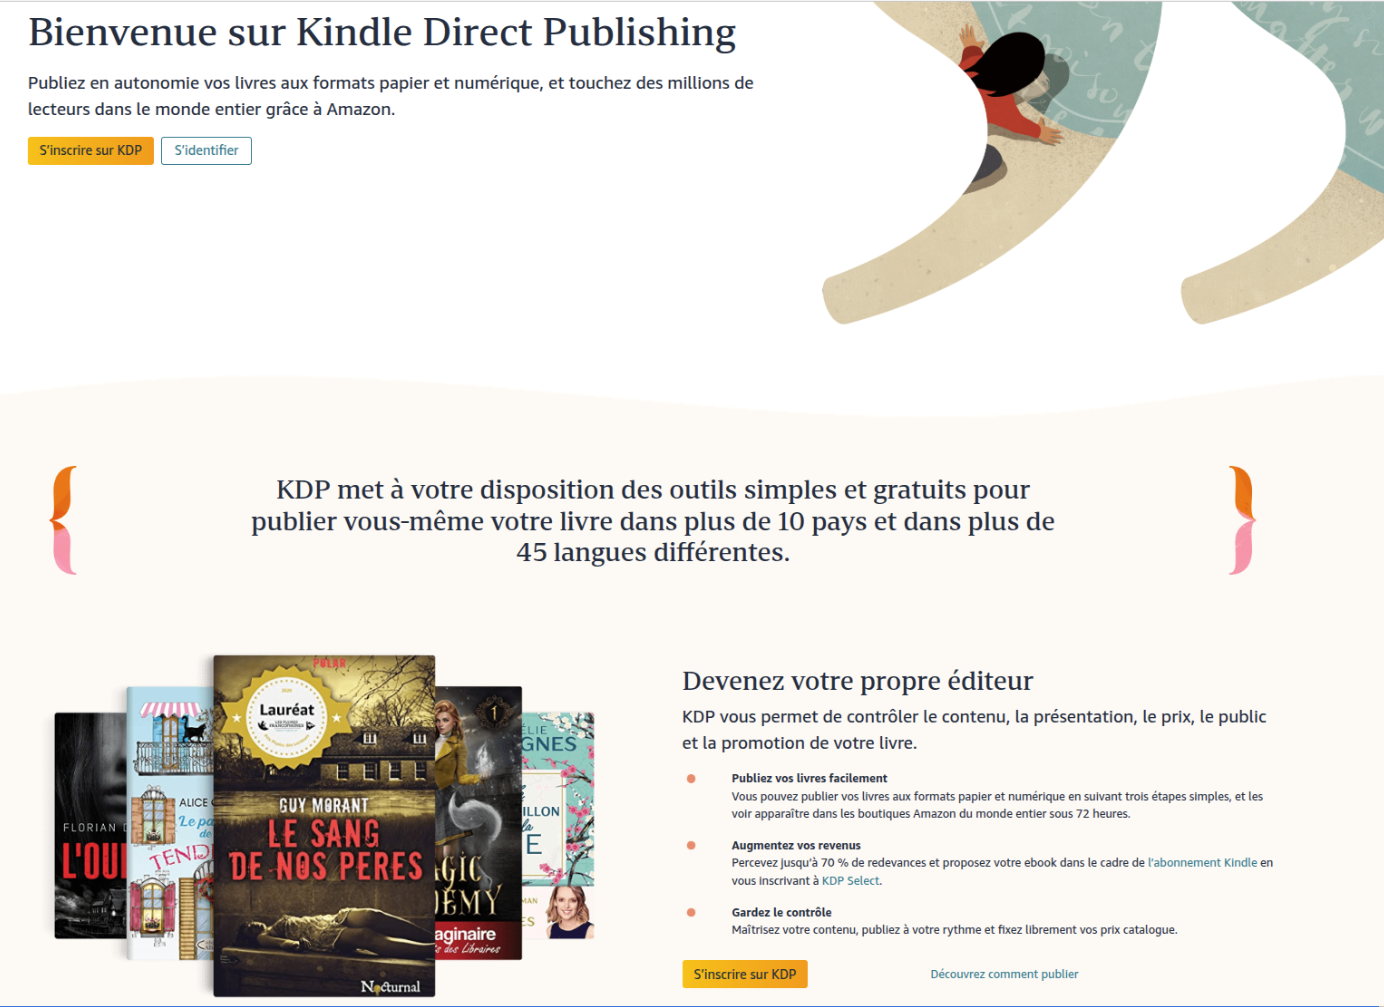
\includegraphics[width=.55\textwidth]{images/kindle_plateforme.png}
\end{figure}
\end{frame}

\begin{frame}{De la désintermédiation à la réintermédiation}
    \begin{columns}
    % Colonne de gauche : Texte
        \begin{column}{0.45\textwidth}
            \begin{itemize}
                \item Depuis juillet 2015, les auteur.rices dont les livres sont empruntés via plateforme ne sont plus rémunéré.es selon le barème d’une base minimale de lecture de 10\% du livre, mais en fonction du nombre de pages lues.
                \item Formatage des écrits pour inciter, coûte que coûte, le lecteur à poursuivre le plus loin possible sa progression dans l’ouvrage ?
            \end{itemize}
        \end{column}

        % Colonne de droite : Image
        \begin{column}{0.5\textwidth}
            \centering
            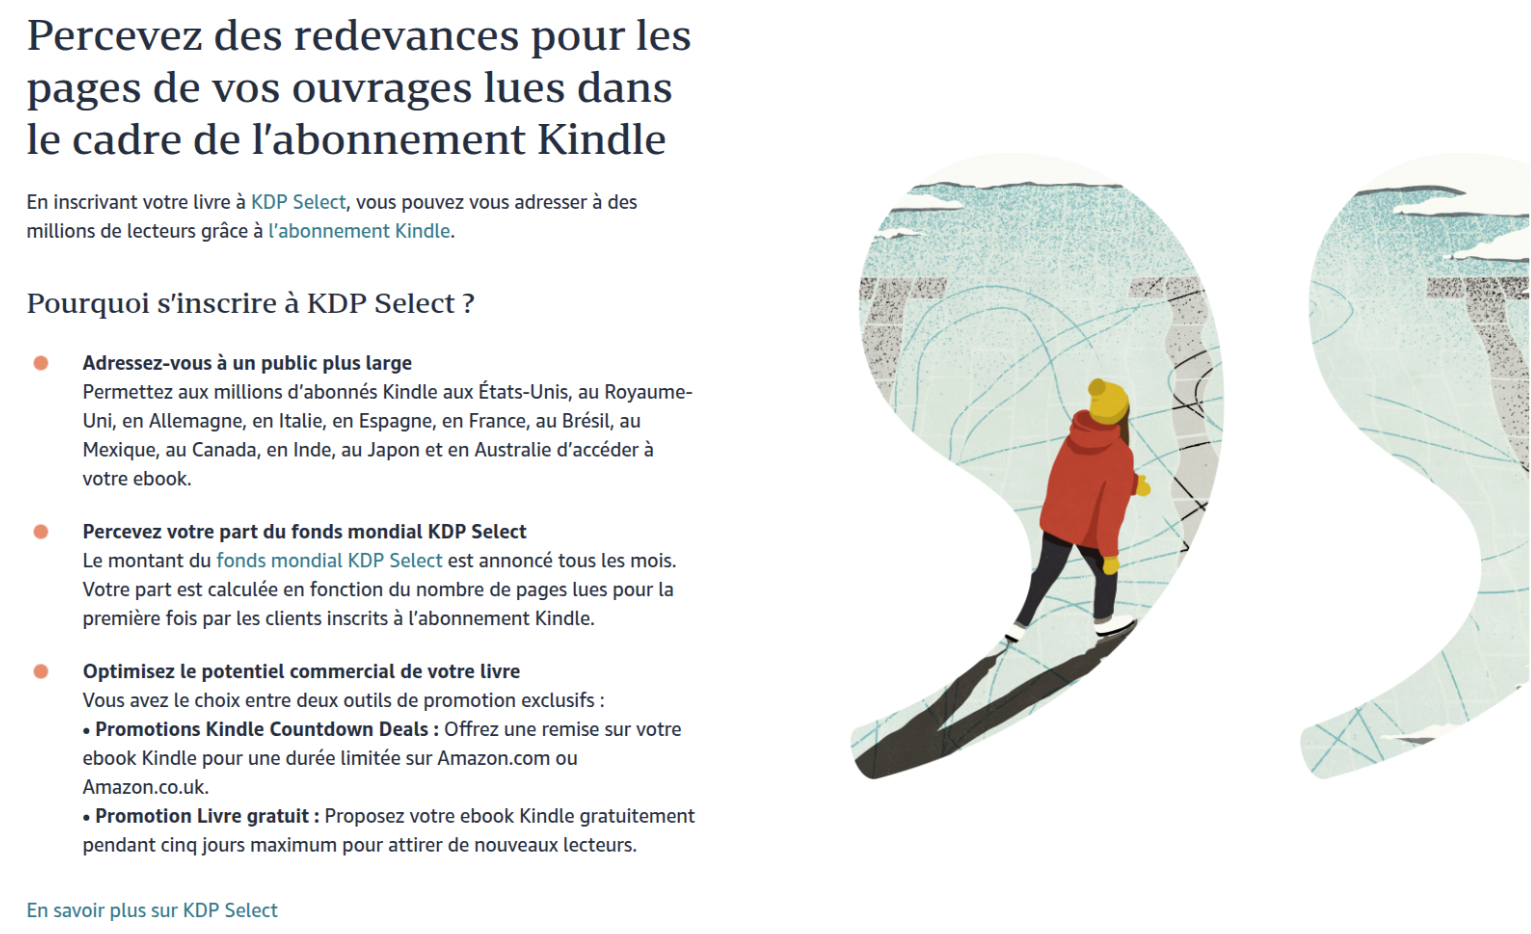
\includegraphics[width=\textwidth]{images/kindle_plateforme2.png}
        \end{column}
    \end{columns}
\end{frame}

\begin{frame}{De la désintermédiation à la réintermédiation}
    \begin{columns}
    % Colonne de gauche : Texte
        \begin{column}{0.4\textwidth}
            \begin{itemize}
                \item \textit{Amazon, par exemple, ne se contente pas de savoir quels livres ses clients achètent sur sa plateforme, il analyse aussi les traces de la vitesse de lecture sur la liseuse : lire le livre en entier ou non, sauter des chapitres, etc.} \textbf{[Dominique Cardon, Culture numérique, 2019]}
            \end{itemize}
        \end{column}

        % Colonne de droite : Image
        \begin{column}{0.5\textwidth}
            \centering
            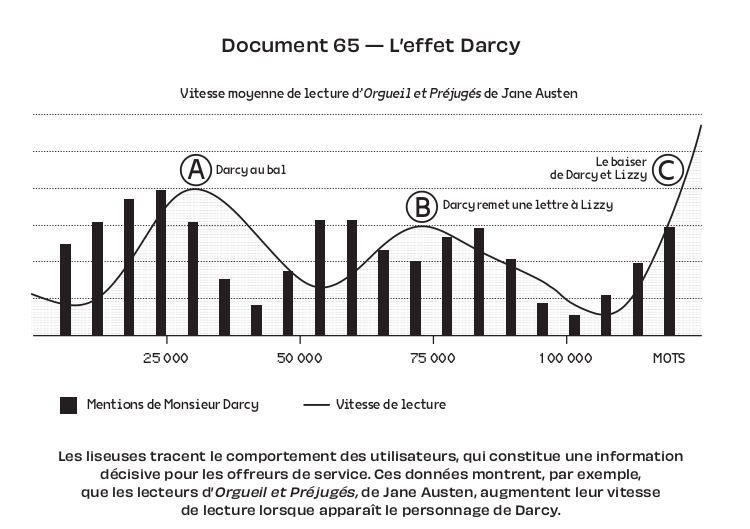
\includegraphics[width=\textwidth]{images/effetDarcy.png}
        \end{column}
    \end{columns}
\end{frame}

\begin{frame}{Réintermédiation numérique : le risque de la plateformisation}
    \textbf{Plateforme = } Logiciels construits par des sociétés à des fins commerciales.\\
    \vspace{1em}
    
    Mounier et Dacos parlent de facteurs de réintermédiation via : 
    \begin{itemize}
        \item le design des plateformes informatiques ;
        \item la définition des règles d'écriture et de lecture ;
        \item la gestion des communautés qui les utilisent ;
        \item les algorithmes de classement de l'information produite.
    \end{itemize}
    \textbf{Plateformisation =} Uniformisation des productions dans un format de publication préconstruit et partagé par une communauté d'utilisateur.rices, avec les dérives potentielles en termes de censure, formatage, appauvrissement de contenu etc...\\
\end{frame}

\section{Conclusion}
\begin{frame}{Conclusion}
  Auto-édition est une pratique ancienne encouragée par certains éditeurs comme Grasset sur \textbf{le principe d'édition à compte d'auteur}.\\
  \textrightarrow{} Entreprises d'auto-édition aujourd'hui portées par des grands noms (Sattouf, Dicker, etc.) concurrencent les maisons d'édition traditionnelles.\\
  \vspace{1em} 
  Une des raisons: \textbf{tensions entre les éditeurs et les auteurs}. Mais attention aux pratiques risquées, portées par des amateurs et jeunes auteurs ou auteurs précaires.\\ 
  \vspace{1em}
  L'auto-édition s'inscrit dans un contexte culturel marqué par un principe de \textbf{désintermédiation} \textrightarrow{} une des principales conséquence est \textbf{la redéfinition de l'autorité des éditeurs}.\\ 
  \vspace{1em}
  Mais l'auto-édition est-elle vraiment synonyme d'émancipation de l'auteur ? Le développement d'un nouveau monopole éditorial basé sur les services numériques (GAFAM), donne lieu à une réintermédiation dont il faut mesurer les effets.
\end{frame}
\end{document}